\section{Storing Groceries [DSPL \& OPL]}
The robot helps by storing newly bought groceries in the cupboard next to the objects of the same kind that are already there; for instance by placing fresh apples where the other apples are.

\subsection{Goal}
The robot has to correctly identify and manipulate objects at different heights, grouping them by category and likelihood.

\subsection{Focus}
This test focuses on the detection and recognition of objects and their features, as well as object manipulation.

\begin{minipage}{0.70\textwidth}
	\subsection{Setup}
	\begin{enumerate}
		\item \textbf{Location:} One of the bookcases or cupboards in the apartment is used for this test, one where a table is near or can be put. 
		\item \textbf{Start position:} The robot will start between the cupboard and the table in a random orientation, but facing towards the Cupboard.
		. 
		\item \textbf{Cupboard:} The cupboard has 5 shelves between 0.30m and 1.80m from the ground and contains several objects (See \ref{rule:scenario_objects}).
		\begin{itemize}
		 	\item \textbf{Door:} The cupboard has a single door, which is closed initially.
		 	This door encloses some of the objects, covering up to one half of the cupboard (e.g. the left or bottom half), as indicated by the hatched area in the image.
		\end{itemize} 
		\item \textbf{Table:} A table near to the Cupboard has 10 objects (See \ref{rule:scenario_objects}). If not all fit the on the table, they will be added during the test. The maximum distance between the Table and the Cupboard is 2m.
		\item \textbf{Objects:} Objects on the Cupboard and on the Table can be known, alike, or unknown. Also, there will be more than one object in each shelf. 
	\end{enumerate}
\end{minipage}\hfill
\begin{minipage}{0.25\textwidth}
	\begin{figure}[H]
		\centering
		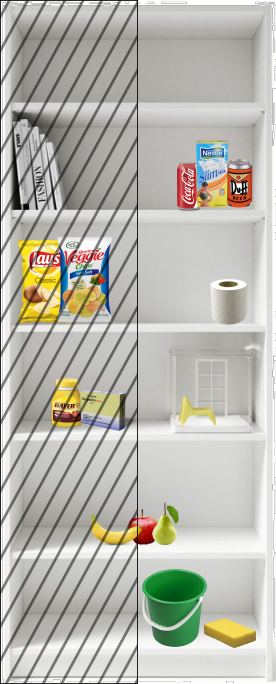
\includegraphics[width=\textwidth]{images/storing_groceries.png}%
		\vspace{-10pt}
		\label{fig:storing_groceries}
		%\caption{Example shelf where objects will be placed.}
		\caption{Shelf}
	\end{figure}
\end{minipage}


\subsection{Task}
\begin{enumerate}
	\item \textbf{Opening door:} The robot starts opening the Cupboard's door. If the robot is unable to open the door, it may ask the Referee to do it instead.
	\item \textbf{Cupboard inspection:} The robot inspects the cupboard locating and categorizing existing groceries.
	\item \textbf{Finding the table:} The turns around and locates the table.  
	\item \textbf{Table inspection:} The robot approaches the table starts analyzing the newly bought groceries (i.e. objects).
	\item \textbf{Moving objects:} The robot chooses which object to move first from the Table to the Cupboard, allocating similar objects all together.
	\begin{itemize}
		\item Objects of the same type (i.e. identical known objects or akin alike objects) must be placed one next to the other.
		\item If the Cupboard has no object of the same type, then objects must be grouped by category (e.g. drinks with drinks, snacks with snacks, etc)
		\item If the Cupboard has no similar object, the robot must clearly state its decision on how to solve the problem. For instance, the robot can define a place for the newly found Category (e.g. Food was found but there is no other food in the cupboard), or group all new objects together (e.g. placing all Unknown objects together).
	\end{itemize}

	\textbf{Note:} Either before or after grasping an object the robot may announce the name of the object found. 
	\item \textbf{Repeat:} This repeats until the time is up or all groceries are stored.
\end{enumerate}

\subsection{Additional rules and remarks}
\begin{enumerate}
	\item \textbf{Bypassing Manipulation:} Bypassing object manipulation via the CONTINUE rule (Section \refsec{rule:asrcontinue}) is not allowed during this test.
	\item \textbf{No setup:} There is no setup time.
	\item \textbf{Startup:} The robot can be started with a simple voice command or via a start button (Section \refsec{rule:start_signal}). 
	\item \textbf{Single try:} The robot must be able to start from the first attempt. There is no restart for this test. If the robot is unable to start it must be removed immediately.
	\item \textbf{Collisions:} Slightly touching the the cupboard is tolerated (but not advised). Crushing objects or any other form of a major collision terminates the test immediately (Section \refsec{rule:safetyfirst}).
	\item \textbf{Recognition report:} Robots must create a PDF report file including
		\begin{enumerate}
			\item The name of the team.
			\item The try number (to identify between runs).
			\item The date and time.
			\item Picture of the cupboard in its initial state with bounding boxes enclosing each group and a human-readable labels to identify them.
			\item The list of moved objects; each one with a picture showing the object inside a bounding box with a label stating the object's name, category, and any other relevant information used to categorize the object.
			\item Picture of the cupboard in its final state with bounding boxes enclosing each group and a human-readable labels to identify them.
		\end{enumerate}

		The report file must be stored on a USB-stick on the robot, which will be collected by the TC immediately after the test. The PDF file must be named with the following format: \texttt{TeamName\_RunNumber.pdf}\\

		\textbf{Remark:} It must be unmistakable which label belongs to which object. Objects must also be easily recognizable in the report by a human (TC) so that it can be scored. \\

		\textbf{Remark:} False positives in the report (labeling an object which is not an object but e.g. the edge of the shelf) are penalized.

		\textbf{Unknown objects:} A significant amount of objects are unknown objects. A correct label for these may be constituted by: 
		\begin{itemize}
			\item Simply labeling those as \quotes{Unknown} as opposed to wrongly applying a label from the known or alike objects
			\item Labeling pairs of unknown objects of the same class with the same label (which may be e.g. \quotes{type\_X} for one pair and \quotes{relevant-feature\_Y} for another). 
			\item Labeling unknown objects with a new, sensible label for objects.
	 	\end{itemize}

	\item \textbf{Clear area:} The robot may assume that the direct vicinity of the cupboard and table are clear, and that the robot can move slightly backwards for its task.
\end{enumerate}

\subsection{Data recording}
Please record the following data (See \refsec{rule:datarecording}):
\begin{itemize}
	\item Images
	\item Plans
\end{itemize}

\subsection{OC instructions}

\textbf{2 hours before the test}
\begin{itemize}
    \item Announce the startup location for robots.
\end{itemize}

\subsection{Referee instructions}
The referee needs to
\begin{itemize}
	\item Place the objects in the cupboard and a few of the same class on the table. New items can be placed when there is room or the robot asks for more objects. 
	\item Close the door of the cupboard. 
	\item Put objects on the table and the corresponding objects in the cupboard: 3 known objects, 2 alike and 5 unknown objects. 
\end{itemize}


\newpage
\subsection{Score sheet}

The maximum time for this test is 3 minutes.

\begin{scorelist}
% There are 5 filled shelves
% On each shelf, there can fit 4 objects: 2 originally there, in the corners. As each object may get a 'companion' put there by the robot, there are 2 more objects per shelf.

% Grasp (any object): 10
% Place (anywhere in the cupboard): 10
% Place in correct place: 15
% Recognize known object correctly (without grasping/placing something of that class): 10
% Label two unknown objects of the same class with the same label (e.g. ``class0''): 15

% Place known object near known object of same class: 40
% Place unknown object near unknown object of the same class: 50


	\scoreheading{Grasping objects}
	\scoreitem[5]{10}{For each successful grasp of any object (lifting it up to at least 5 cm for more than 10 seconds)}

	\scoreheading{Placing objects}
	\scoreitem[5]{10}{For each successful placement of an object anywhere in the cupboard (safely stands still for more than 10 seconds)}
	\scoreitem[5]{5}{For each successful placement of an object at correct place (near an object of the same class)}

	\scoreheading{Recognizing objects}
	\scoreitem[5]{10}{Every correctly recognized known or alike object in the report file}
	\scoreitem[5]{15}{Corresponding labels for pairs of unknown objects of the same class, in the report file 
            \footnote{Suppose there is a rubber ducky as an unknown object class. Two rubber duckies must be given the same label (e.g. ``label0'') to receive these points}}
	\scoreitem[5]{-5}{False positive label}
	
% 	\scoreheading{Total task}
% 	\scoreitem[5]{40}{Place known object near known object of same class}
% 	\scoreitem[5]{50}{Place unknown object near unknown object of same class}

	\scoreheading{Bonus}
	\scoreitem[1]{20}{Open the door without human help}
	
	\setTotalScore{250}
\end{scorelist}


% Local Variables:
% TeX-master: "Rulebook"
% End:


% Local Variables:
% TeX-master: "Rulebook"
% End:
